%%%%%%%%%%%%%%%%%%%%%%%%%%%%%%%%%%%%%%%%%
% Lachaise Assignment
% LaTeX Template
% Version 1.0 (26/6/2018)
%
% This template originates from:
% http://www.LaTeXTemplates.com
%
% Authors:
% Marion Lachaise & François Févotte
% Vel (vel@LaTeXTemplates.com)
%
% License:
% CC BY-NC-SA 3.0 (http://creativecommons.org/licenses/by-nc-sa/3.0/)
% 
%%%%%%%%%%%%%%%%%%%%%%%%%%%%%%%%%%%%%%%%%

%----------------------------------------------------------------------------------------
%	PACKAGES AND OTHER DOCUMENT CONFIGURATIONS
%----------------------------------------------------------------------------------------

\documentclass{article}

%%%%%%%%%%%%%%%%%%%%%%%%%%%%%%%%%%%%%%%%%
% Lachaise Assignment
% Structure Specification File
% Version 1.0 (26/6/2018)
%
% This template originates from:
% http://www.LaTeXTemplates.com
%
% Authors:
% Marion Lachaise & François Févotte
% Vel (vel@LaTeXTemplates.com)
%
% License:
% CC BY-NC-SA 3.0 (http://creativecommons.org/licenses/by-nc-sa/3.0/)
% 
%%%%%%%%%%%%%%%%%%%%%%%%%%%%%%%%%%%%%%%%%

%----------------------------------------------------------------------------------------
%	PACKAGES AND OTHER DOCUMENT CONFIGURATIONS
%----------------------------------------------------------------------------------------

\usepackage{amsmath,amsfonts,stmaryrd,amssymb} % Math packages

\usepackage{enumerate} % Custom item numbers for enumerations

\usepackage[ruled]{algorithm2e} % Algorithms

\usepackage[framemethod=tikz]{mdframed} % Allows defining custom boxed/framed environments

\usepackage{listings} % File listings, with syntax highlighting
\lstset{
	basicstyle=\ttfamily, % Typeset listings in monospace font
}

\usepackage[hidelinks,colorlinks=true]{hyperref}

%----------------------------------------------------------------------------------------
%	DOCUMENT MARGINS
%----------------------------------------------------------------------------------------

\usepackage{geometry} % Required for adjusting page dimensions and margins

\geometry{
	paper=a4paper, % Paper size, change to letterpaper for US letter size
	top=2.5cm, % Top margin
	bottom=3cm, % Bottom margin
	left=2.5cm, % Left margin
	right=2.5cm, % Right margin
	headheight=14pt, % Header height
	footskip=1.5cm, % Space from the bottom margin to the baseline of the footer
	headsep=1.2cm, % Space from the top margin to the baseline of the header
	%showframe, % Uncomment to show how the type block is set on the page
}

%----------------------------------------------------------------------------------------
%	FONTS
%----------------------------------------------------------------------------------------

\usepackage[utf8]{inputenc} % Required for inputting international characters
\usepackage[T1]{fontenc} % Output font encoding for international characters

%\usepackage{XCharter} % Use the XCharter fonts

%----------------------------------------------------------------------------------------
%	COMMAND LINE ENVIRONMENT
%----------------------------------------------------------------------------------------

% Usage:
% \begin{commandline}
%	\begin{verbatim}
%		$ ls
%		
%		Applications	Desktop	...
%	\end{verbatim}
% \end{commandline}

\mdfdefinestyle{commandline}{
	leftmargin=10pt,
	rightmargin=10pt,
	innerleftmargin=15pt,
	middlelinecolor=black!50!white,
	middlelinewidth=2pt,
	frametitlerule=false,
	backgroundcolor=black!5!white,
	frametitle={Command Line},
	frametitlefont={\normalfont\sffamily\color{white}\hspace{-1em}},
	frametitlebackgroundcolor=black!50!white,
	nobreak,
}

% Define a custom environment for command-line snapshots
\newenvironment{commandline}{
	\medskip
	\begin{mdframed}[style=commandline]
}{
	\end{mdframed}
	\medskip
}

%----------------------------------------------------------------------------------------
%	FILE CONTENTS ENVIRONMENT
%----------------------------------------------------------------------------------------

% Usage:
% \begin{file}[optional filename, defaults to "File"]
%	File contents, for example, with a listings environment
% \end{file}

\mdfdefinestyle{file}{
	innertopmargin=1.6\baselineskip,
	innerbottommargin=0.8\baselineskip,
	topline=false, bottomline=false,
	leftline=false, rightline=false,
	leftmargin=2cm,
	rightmargin=2cm,
	singleextra={%
		\draw[fill=black!10!white](P)++(0,-1.2em)rectangle(P-|O);
		\node[anchor=north west]
		at(P-|O){\ttfamily\mdfilename};
		%
		\def\l{3em}
		\draw(O-|P)++(-\l,0)--++(\l,\l)--(P)--(P-|O)--(O)--cycle;
		\draw(O-|P)++(-\l,0)--++(0,\l)--++(\l,0);
	},
	nobreak,
}

% Define a custom environment for file contents
\newenvironment{file}[1][File]{ % Set the default filename to "File"
	\medskip
	\newcommand{\mdfilename}{#1}
	\begin{mdframed}[style=file]
}{
	\end{mdframed}
	\medskip
}

%----------------------------------------------------------------------------------------
%	NUMBERED QUESTIONS ENVIRONMENT
%----------------------------------------------------------------------------------------

% Usage:
% \begin{question}[optional title]
%	Question contents
% \end{question}

\mdfdefinestyle{question}{
	innertopmargin=1.2\baselineskip,
	innerbottommargin=0.8\baselineskip,
	roundcorner=5pt,
	nobreak,
	singleextra={%
		\draw(P-|O)node[xshift=1em,anchor=west,fill=white,draw,rounded corners=5pt]{%
		Question \theQuestion\questionTitle};
	},
}

\newcounter{Question} % Stores the current question number that gets iterated with each new question

% Define a custom environment for numbered questions
\newenvironment{question}[1][\unskip]{
	\bigskip
	\stepcounter{Question}
	\newcommand{\questionTitle}{~#1}
	\begin{mdframed}[style=question]
}{
	\end{mdframed}
	\medskip
}

%----------------------------------------------------------------------------------------
%	WARNING TEXT ENVIRONMENT
%----------------------------------------------------------------------------------------

% Usage:
% \begin{warn}[optional title, defaults to "Warning:"]
%	Contents
% \end{warn}

\mdfdefinestyle{warning}{
	topline=false, bottomline=false,
	leftline=false, rightline=false,
	nobreak,
	singleextra={%
		\draw(P-|O)++(-0.5em,0)node(tmp1){};
		\draw(P-|O)++(0.5em,0)node(tmp2){};
		\fill[black,rotate around={45:(P-|O)}](tmp1)rectangle(tmp2);
		\node at(P-|O){\color{white}\scriptsize\bf !};
		\draw[very thick](P-|O)++(0,-1em)--(O);%--(O-|P);
	}
}

% Define a custom environment for warning text
\newenvironment{warn}[1][Warning:]{ % Set the default warning to "Warning:"
	\medskip
	\begin{mdframed}[style=warning]
		\noindent{\textbf{#1}}
}{
	\end{mdframed}
}

%----------------------------------------------------------------------------------------
%	INFORMATION ENVIRONMENT
%----------------------------------------------------------------------------------------

% Usage:
% \begin{info}[optional title, defaults to "Info:"]
% 	contents
% 	\end{info}

\mdfdefinestyle{info}{%
	topline=false, bottomline=false,
	leftline=false, rightline=false,
	nobreak,
	singleextra={%
		\fill[black](P-|O)circle[radius=0.4em];
		\node at(P-|O){\color{white}\scriptsize\bf i};
		\draw[very thick](P-|O)++(0,-0.8em)--(O);%--(O-|P);
	}
}

% Define a custom environment for information
\newenvironment{info}[1][Info:]{ % Set the default title to "Info:"
	\medskip
	\begin{mdframed}[style=info]
		\noindent{\textbf{#1}}
}{
	\end{mdframed}
}

 % Include the file specifying the document structure and custom commands

%----------------------------------------------------------------------------------------
%	ASSIGNMENT INFORMATION
%----------------------------------------------------------------------------------------

\title{T-10 paper simulation} % Title of the assignment

\author{John Brooks\\ \texttt{jwb2159@columbia.edu}} % Author name and email address

\date{Columbia University --- \today} % University, school and/or department name(s) and a date

%----------------------------------------------------------------------------------------

\begin{document}

\maketitle % Print the title

%----------------------------------------------------------------------------------------
%	INTRODUCTION
%----------------------------------------------------------------------------------------

\section{Introduction} % Unnumbered section

This writeup covers the derivation implementation of Chudnovskiy's 2003 tearing mode simulation on the T-10 tokamak with a biased limiter \cite{2003}.  Some of the details I needed to fully implement the simulation were missing, and a later T-10 paper by Ivanov \cite{2014} fills in some of the gaps.  

The code solves for the perturbed magnetic poloidal flux $\Psi(r,t)$ in the T-10 tokamak in the presence of m/n=2/1 tearing mode and with a biased limiter.  The idea of the simulation is that current sourced by the biased limiter into the plasma couples with the tearing mode and can result it changes in the mode's amplitude and frequency\cite{2003}.    




\section{Code setup} % Numbered section

The domain for this problem is broken up into three sections: the region inside the resonant surface ($0<r<r_s-W/2$), the resonant surface ($r_s-W/2<r<r_s+W/2$ and the region outside ($r_s+W/2<r<b$) where $r_s$ is the location of the resonant surface, $W$ is the island width, and $b$ is the location of the vessel wall and magnetic sensor.  

The inner and outer regions are a Boundary Value Problem (BVP) with a current source term at $a$, the location of the limiter.  The middle region is a time evolution problem of the tearing mode solved at $r_s$, and $\Psi$ within this region is assumed to be constant.  The middle region couples to the outer regions by providing Dirichlet boundary conditions to the BVPs.  In return, the BVPs dictate the tearing mode stability parameter which is needed to calculate the time evolution of the tearing mode.   

\subsection{Boundary Value Problem (BVP)}


The BVP equations take the form,


\begin{equation} \label{eq:BVPEquations}
\begin{split}
\frac{\partial}{\partial r} &  \left( r \frac{\partial \Psi_C}{\partial r} \right)-\left( \frac{m^2}{r} +\frac{\mu_0 R}{B_T} \frac{\partial j / \partial r}{\mu(r)-n/m} \right) \Psi_C  = - \mu_0r \cdot \iota(t) \delta (r-a)  \\
 \frac{\partial}{\partial r} &  \left( r \frac{\partial \Psi_S}{\partial r} \right)-\left( \frac{m^2}{r} +\frac{\mu_0 R}{B_T} \frac{\partial j / \partial r}{\mu(r)-n/m} \right) \Psi_S =0
\end{split}
\end{equation}

\noindent where the $C$ and $S$ subscripts represent the cosine and sine components of $\Psi$.  These equations need to be solved for both the sine and cosine terms and in the inner and outer regions, resulting in 4 BVP equations.  Of note, $W$ is a function of time and grows and contracts as the island expands and contracts.  This results in the sizes of the three domains periodically expanding and contracting, making the solver more complicated.   

To solve Eq.~\ref{eq:BVPEquations}, it first needs to be discretized.  Of note, there , and there are four versions of this equation (inner cosine, inner sine, outer cosine, and outer sine).  Fortunately, the discretized form is nearly identical:


\begin{equation} \label{eq:BVPSolved}
\begin{split}
 \frac{\partial \Psi^n}{\partial r} + r \frac{\partial^2 \Psi^n}{\partial r^2} -\alpha(r)  \Psi^n  & = - \beta(r,t) \\ 
 \frac{\Psi^{n+1}-\Psi^{n-1}}{2\Delta r}+r\left(\frac{\Psi^{n+1}-2\Psi^{n}+\Psi^{n-1}}{\Delta r^2}\right)-\alpha(r)\Psi^n & = - \beta(r,t)  \\
  \Psi^{n+1}\left(\frac{1}{2 \Delta r}+\frac{r}{\Delta r^2 }\right) + \Psi^n\left( \frac{-2r}{\Delta r^2} -\alpha(r) \right) + \Psi^{n-1}\left(-\frac{1}{2\Delta r} + \frac{r}{\Delta r^2} \right) & = - \beta(r,t) \\
  \Psi^{n+1} \ \gamma_{+1}(r) + \Psi^n \ \gamma_{0}(r) + \Psi^{n-1} \ \gamma_{-1}(r) & = - \beta(r,t) \\
A(r) \Psi(r) & = -\beta(r,t) \\
\end{split}
\end{equation}

\noindent and $\Psi$ is solved with python's \emph{scipy.sparse.linalg.spsolve} command.  

The boundary conditions for $\Psi$ are

\begin{equation} \label{eq:BVPAMatrix}
\begin{split}
\Psi_{C,S}(0)&=0 \\
\Psi_{C,S}(b)&=0 \\
\Psi_{C,S}(r_s-W/2)&=\Psi_{C,S}(t,r_s) \\
\Psi_{C,S}(r_s+W/2)&=\Psi_{C,S}(t,r_s) \\
\end{split}
\end{equation}

\noindent where $\Psi_{C,S}(r_s)$ is time evolution of $\Psi$ solved at the surface and discussed in the following section.  To enforce these boundary conditions, $A$ and $\beta_{C,S}$ need to be set correctly.  For $A$, the on-diagonal corner entries are set to 1, 

\begin{equation} \label{eq:BVPAMatrix}
\begin{split}
A &= 
\begin{bmatrix}
1& 0 & 0 & & & & 0\\
 \gamma_{-1}(r)  & \gamma_{0}(r)      & \gamma_{+1}(r) &  &   &  \\
0 & \gamma_{-1}(r)       & \gamma_{0}(r)      & \gamma_{+1}(r)  &  &  \\
& & \ddots      & \ddots  & \ddots  & \\
& &    &\gamma_{-1}(r)       & \gamma_{0}(r)      & \gamma_{+1}(r) & 0 \\
&        &  &  & \gamma_{-1}(r)       & \gamma_{0}(r) & \gamma_{+1}(r) \\
0 &        &  &  & 0 &  0  & 1 \\
\end{bmatrix}. \\
\end{split}
\end{equation}

Above, the continuous form of $\beta$ is

\begin{equation} \label{eq:beta}
\begin{split}
\beta(r,t) &= \left\{
\begin{array}{l l}
\mu_0r \cdot \iota(t) \delta (r-a) & \text{ for } \Psi_C \\
0 & \text{ for } \Psi_S\\
\end{array} \right. \\\
\end{split}
\end{equation} 
and it needs to be solved for all four $\Psi$ terms.  In addition, the first and last terms in $\beta$ contain the BC values discussed above.  Therefore, it's discretized form is
\begin{equation} \label{eq:BVPAMatrix}
\begin{split}
\beta_{C \ inside}(t) &= 
\begin{bmatrix}
0,& \ldots &  0, & \Psi_{C}(t,r_s)
\end{bmatrix}^T, \\
\beta_{S \ inside}(t) &= 
\begin{bmatrix}
0,& \ldots &  0, & \Psi_{S}(t,r_s)
\end{bmatrix}^T, \\
\beta_{C \ outside}(t) &= 
\begin{bmatrix}
\Psi_{C}(t,r_s), & 0, & \ldots &0, &\mu_0r_s \cdot \iota(t)/\Delta r,  &0,&\ldots &  0 
\end{bmatrix}^T, \\
\beta_{S \ outside}(t) &= 
\begin{bmatrix}
\Psi_{S}(t,r_s), & 0, & \ldots &  0 \\
\end{bmatrix}^T, \\
\end{split}
\end{equation}
where the discretized delta function is $1/ \Delta r$ and is defined only at the $r=r_s$ grid.  Here, $\Delta r$ is the width of each radial grid.


The other terms in the above equations are

\begin{equation} \label{eq:BVPTerms}
\begin{split}
\alpha(r)&=\left( \frac{m^2}{r} +\frac{\mu_0 R}{B_T} \frac{\partial j / \partial r}{\mu(r)-n/m} \right) \\
\mu(r)&=1/q(r)\\
\iota(t) &= \frac{J(t)m}{2a} \\
  \gamma_{+1}(r) &=\left(\frac{1}{2 \Delta r}+\frac{r}{\Delta r^2 }\right) \\
  \gamma_{0}(r)& = \left( \frac{-2r}{\Delta r^2} -\alpha(r) \right)\\
  \gamma_{-1}(r)& = \left(-\frac{1}{2\Delta r} + \frac{r}{\Delta r^2} \right)
\end{split}
\end{equation}

In addition, first order center differencing was used to discretize the differential operators.  

\begin{equation} \label{eq3}
\begin{split}
 \frac{\partial f^n}{\partial x} & = \frac{f^{n+1}-f^{n-1}}{2\Delta x} \\
 \frac{\partial^2 f^n}{\partial x^2} & = \frac{f^{n+1}-2f^n+f^{n-1}}{\Delta x^2} \\
\end{split} 
\end{equation} 


\subsection{Time step}

The BVP problem, discussed in the previous section, is solved for the domain inside of the rational surface and outside of the rational surface.  The time evolution of the tearing mode only occurs at $r_s$ and is evolved in time with a first order forward Euler step.  The solution for each time advance provides the boundary conditions for the BVPs which then need to be resolved and then the time advanced again.  

The tearing modes evolution equations are

\begin{equation} \label{eq3}
\begin{split}
 & \frac{\partial \Psi_{C,r_s}}{\partial t} =k a^2 \omega_R \frac{\Delta'_C(W)}{W}\Psi_{C,r_s}-\Omega \Psi_{S,r_s} \\
  & \frac{\partial \Psi_{S,r_s}}{\partial t} =k a^2 \omega_R \frac{\Delta'_S(W)}{W}\Psi_{S,r_s}-\Omega \Psi_{C,r_s}
\end{split} 
\end{equation} 

Discretizing and solving, it takes the form


\begin{equation} \label{eq3}
\begin{split}
\frac{\Psi_{C,r_s}^{n+1}-\Psi_{C,r_s}^{n}}{\Delta t} &=\left( k a^2 \omega_R \frac{\Delta'^{\ n}_{C}(W^n)}{W^n}\Psi_{C,r_s}^n-\Omega \Psi_{S,r_s}^n  \right ) \\
\Psi_{C,r_s}^{n+1} &=\Psi_{C,r_s}^{n}+\Delta t \left( k a^2 \omega_R \frac{\Delta'^{\ n}_C(W^{n})}{W^{n}}\Psi_{C,r_s}^{n}-\Omega \Psi_{S,r_s}^{n} \right )  \\ 
\Psi_{C,r_s}^{n+1} &=\Psi_{C,r_s}^{n}\left( 1 + \Delta t  k a^2 \omega_R \frac{\Delta'^{\ n}_C(W^{n})}{W^{n}}\right) - \Delta t \Omega \Psi_{S,r_s}^{n}   \\
\Psi_{C,r_s}^{n+1} &=\Psi_{C,r_s}^{n}\left( 1 + \zeta \frac{\Delta'^{\ n}_C(W^{n})}{W^{n}}\right) - \eta \Psi_{S,r_s}^{n}   \\
\end{split} 
\end{equation} 

where



\begin{equation} \label{eq3}
\begin{split}
 & W(r_s) = 4 \sqrt{\frac{\sqrt{\Psi^2_{C,r_s} + \Psi^2_{S,r_s}}}{-r_sB_T\mu'(r_s)/R} }\\
  & \Delta'_{C,S}(W)=\frac{\Psi'_{C,S}(r_s+W/2)-\Psi'_{C,S}(r_s-W/2)}{\Psi_{C,S}} \\
  & \zeta = \Delta t k a^2 \omega_R \\
  & \eta =  \Delta t \Omega \\
\end{split} 
\end{equation} 

Note that the prime symbol ($'$) is the radial derivative.  


\section{Initial Conditions}

The 2003 T-10 paper is a little vague in many regards but especially when it comes to its ICs.  Fortunately, a 2014 T-10 paper provides more details, but it is unclear if they are the same ICs that the 2003 paper used.  Below, I summarize the ICs that I'm using. 

\begin{equation} \label{ICConstants}
\begin{split}
m &= 2 \\
n &= 1 \\
R &= 1.5 \ \text{m}\\
B_T &= 2.5 \ \text{T} \\
I_p &= 250e3 \ \text{A}\\
\Omega & =1e3 \ \text{Hz} \cdot 2 \pi \\
\omega_r & = 1/0.01 \ \text{Hz} \\
k &= \pi \\
b = r_{wall} & = 0.39 \ \text{m} \\
a = r_{limiter} & = 0.27 \ \text{m} \\
q(0) &= 0.7/0.85 \\
q(a) = q(r_{limiter}) &= 2.4 \\
B(b) = B(r_{wall}) & = 5e-4 \ \text{T}
\end{split} 
\end{equation} 

The functions used for $q$ and $j$ were unclear in the 2003 paper.  In fact, it states ``The plasma current pofile used in calculatio nwas adjusted to produce the saturated m=2 mode amplitude of 5e-4 T without the external helical current'' which isn't very helpful.  The 2014 paper suggests some possibilities.  

\begin{equation} \label{wessonCurrentProfile}
\begin{split}
j(r)=j(0) \left[ 1-(r/a)^2 \right]^l
\end{split} 
\end{equation} 

\noindent where 

\begin{equation} \label{j}
\begin{split}
l=\left[ q(a)/q(0)\right]-1 = 1.914
\end{split} 
\end{equation} 

Because $j(0)$ was not provided but $I_p$ was, the above model for $j(r)$ was used, integrated $I_p = 2\pi \int_0^b j(r)r \ dr$ and compared with the provided $I_p$ until the correct $j(0)$ was found.  This provided the following profile and its derivative.


\begin{figure}[htb]
	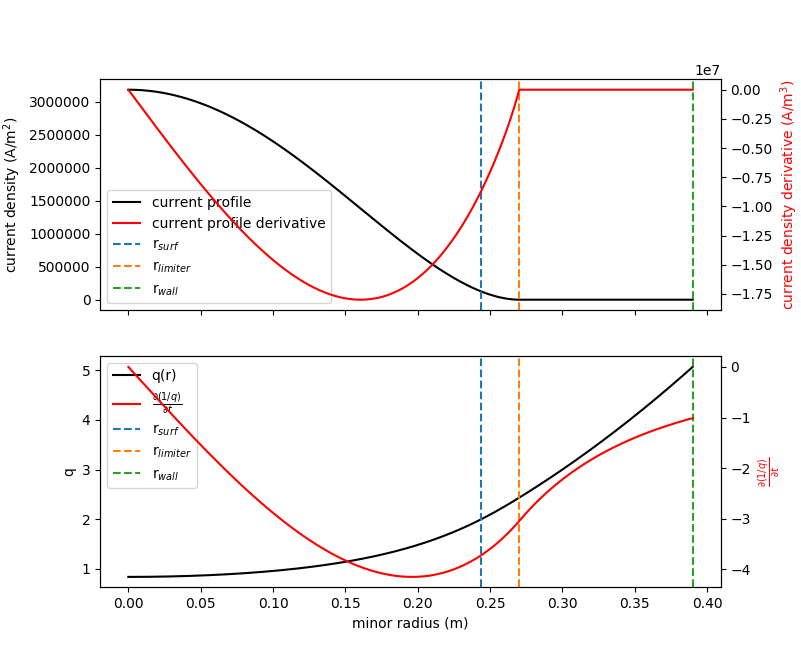
\includegraphics[width=15cm]{images/jAndQ.png}
	\caption{Current and q profile
		\label{fig:jAndQ}}    
\end{figure}  

\noindent Possibly $q(0)$ and $q(a)$ could be adjusted to get slightly different current profiles.  


The q-profile is a little more difficult.  The 2003 paper made no mention other than constraining $q(0)$ and $q(a)$.  The 2014 paper suggested the cylindrical approximation

\begin{equation} \label{qCylindrical}
\begin{split}
q_{cyl}(r\leq a)=\frac{2(l+1)B_T}{\mu_0 j(0) R} \frac{(r/a)^2}{1-\left[ 1-(r/a)^2\right]^{l+1}}.
\end{split} 
\end{equation} 
However, this equation is not valid for $r>a$.  To solve for $q(r>a)$, I combined $\oint B_{\theta} dl = \mu_0 I_p$ and $q=\frac{rB_T}{RB_{\theta}}$ to get 
\begin{equation} \label{qCylindrical}
\begin{split}
q(r>a)=\frac{2\pi r^2B_T}{R\mu_0I_p}
\end{split} 
\end{equation} 
Fig.~\ref{fig:jAndQ}b shows $q(r)$ and the radial derivative of $1/q(r)$.  





%----------------------------------------------------------------------------------------
%	PROBLEM 2
%----------------------------------------------------------------------------------------


% %\bibliographystyle{plain}
% %\bibliography{bibFile.bib}
\bibliographystyle{apsrev}% ,isbn=false %[isbn=false]
\begin{thebibliography}{}

\bibitem{2003}
A. Chudnovskiy, Y. Gvozdkov, N. Ivanov, et. al.,
\emph{Nuclear Fusion}
{\bf 43} (2003). 

\bibitem{2014}
N. V. Ivanov, A.M. Kakurin,
\emph{Physics of Plasmas}
{\bf 21}, 102502 (2014). 


\end{thebibliography}

%----------------------------------------------------------------------------------------

\end{document}

